\subsection{Giao diện của ứng dụng khi khởi động}
Khi mở ứng dụng, giao diện ban đầu của ứng dụng là màn hình đăng nhập, ở đây ta có thể đăng nhập với 2 vai trò đó là User bình thường (Server) hoặc Admin (Client). Mặc định thì ứng dụng sẽ hiển thị ô đăng nhập với vai trò là User, để đăng nhập với vai trò Admin thì ta tích vào ô ``\textbf{Login as ADMIN}``. (Hình \ref{fig:ServerLogin} và Hình \ref{fig:ClientLogin})

\begin{figure}[H]
	\centering{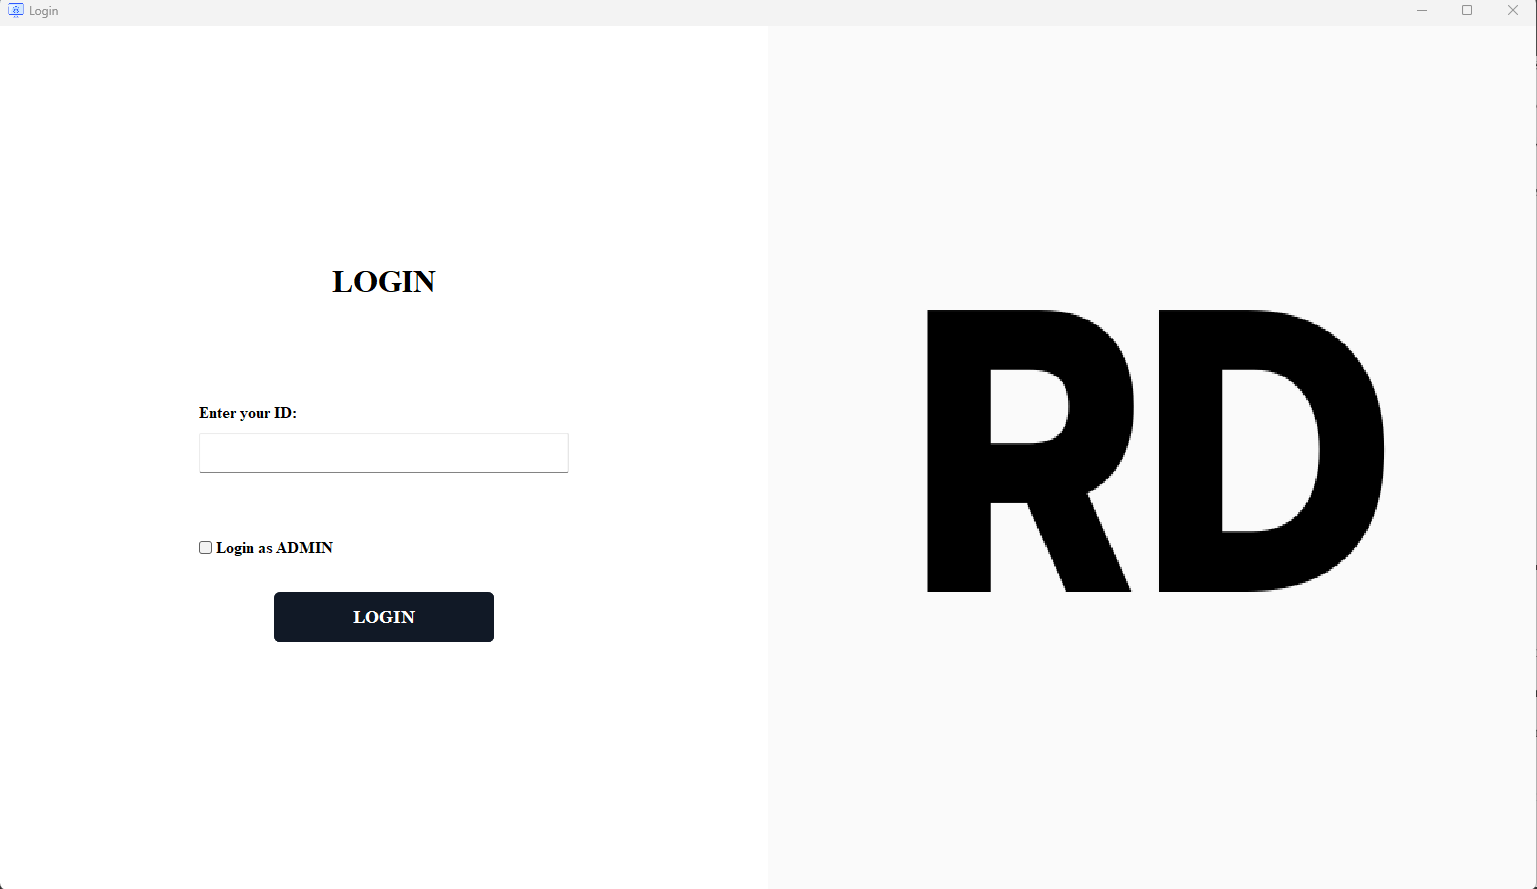
\includegraphics[scale=0.35]{ServerLoginWindow}}
	\caption{Màn hình đăng nhập của User}
	\label{fig:ServerLogin}
\end{figure}

\begin{figure}[H]
	\centering{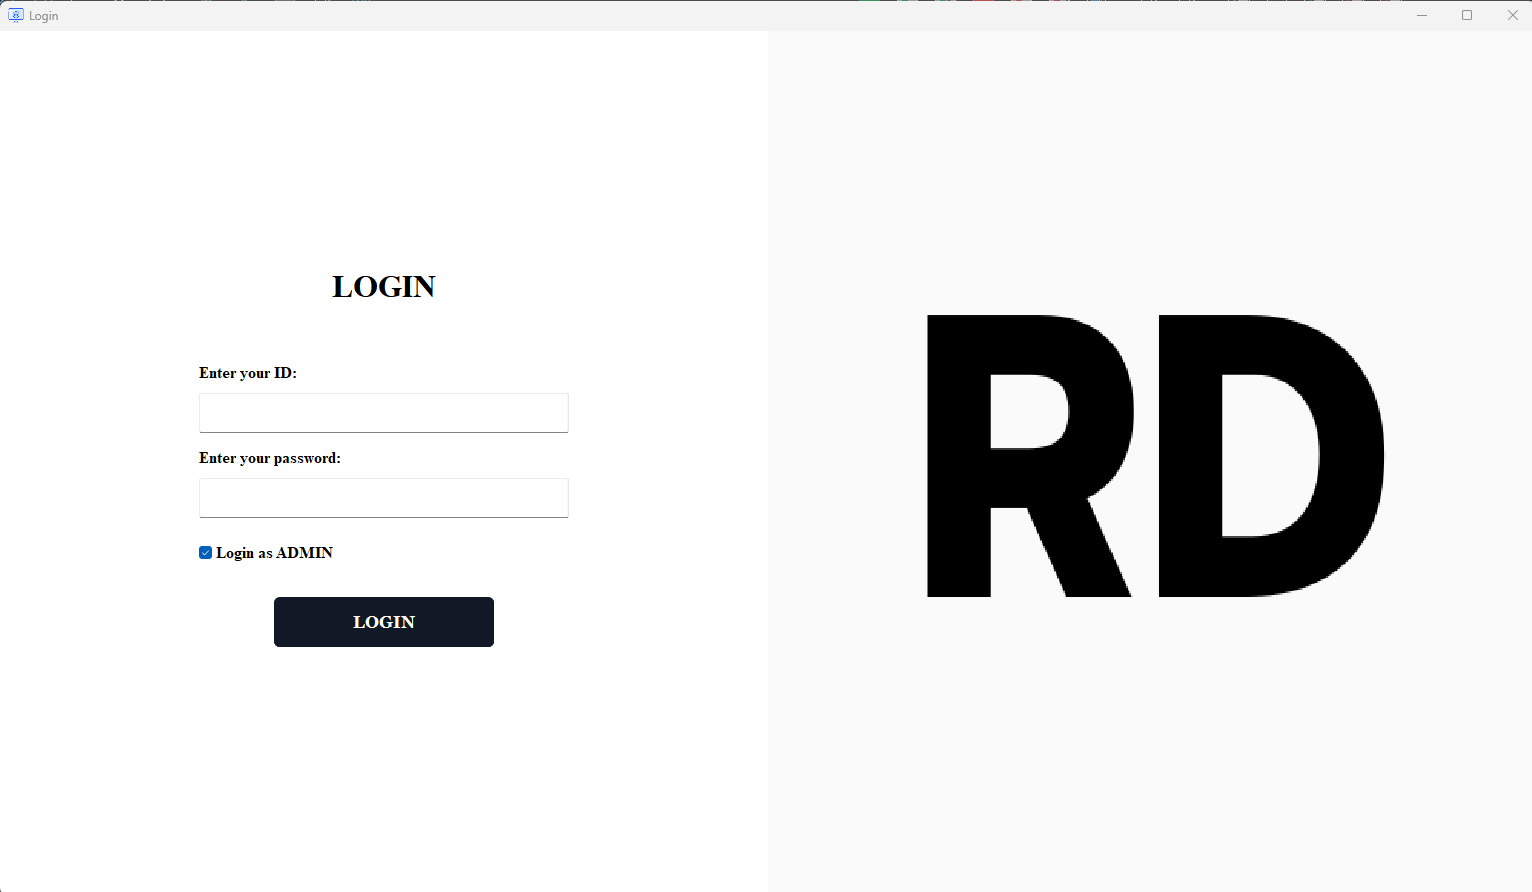
\includegraphics[scale=0.35]{ClientLoginWindow}}
	\caption{Màn hình đăng nhập của Admin}
	\label{fig:ClientLogin}
\end{figure}

Để đăng nhập được với vai trò là User, ta cần nhập tên đăng nhập là một chuỗi ký tự ASCII với độ dài từ 4 đến 10 ký tự. Còn đối với Admin thì tên đăng nhập và mật khẩu mặc định là \verb|admin|.
\subsubsection{Các hàm đã cài đặt}
Hello